%% LyX 2.0.6 created this file.  For more info, see http://www.lyx.org/.
%% Do not edit unless you really know what you are doing.
\documentclass[11pt]{article}
\usepackage[utf8]{inputenc}
\usepackage{prettyref}
\usepackage{amsthm}
\usepackage{amsmath}
\usepackage{amssymb}
\usepackage{graphicx}
\usepackage{esint}
\usepackage[unicode=true,pdfusetitle,
 bookmarks=true,bookmarksnumbered=false,bookmarksopen=false,
 breaklinks=false,pdfborder={0 0 1},backref=section,colorlinks=false]
 {hyperref}
\hypersetup{
 colorlinks,citecolor=blue,urlcolor=blue,linkcolor=blue}

\makeatletter
%%%%%%%%%%%%%%%%%%%%%%%%%%%%%% Textclass specific LaTeX commands.
\theoremstyle{plain}
\newtheorem{thm}{\protect\theoremname}
  \theoremstyle{definition}
  \newtheorem{example}[thm]{\protect\examplename}
 \theoremstyle{definition}
 \newtheorem*{defn*}{\protect\definitionname}
  \theoremstyle{definition}
  \newtheorem{defn}[thm]{\protect\definitionname}

%%%%%%%%%%%%%%%%%%%%%%%%%%%%%% User specified LaTeX commands.
% Borrowed from MIT 6.987 Advanced Data Structures course (Prof Demaine, 2003)


\usepackage{amsthm}\usepackage{bm}\usepackage[usenames,dvipsnames]{xcolor}\usepackage{hypernat}

\usepackage{tikz}\usepackage{tkz-graph}

\newcommand{\handout}[5]{
  \noindent
  \begin{center}
  \framebox{
    \vbox{
      \hbox to 5.78in { {\bf STA4513: Statistical Models of Networks } \hfill #2 }
      \vspace{4mm}
      \hbox to 5.78in { {\Large \hfill #5  \hfill} }
      \vspace{2mm}
      \hbox to 5.78in { {\em #3 \hfill #4} }
    }
  }
  \end{center}
  \vspace*{4mm}
}

\newcommand{\lecture}[4]{\handout{#1}{#2}{#3}{Scribe: #4}{Lecture #1}}

\newtheorem{theorem}{Theorem}
\newtheorem{corollary}[theorem]{Corollary}
\newtheorem{lemma}[theorem]{Lemma}
\newtheorem{observation}[theorem]{Observation}
\newtheorem{proposition}[theorem]{Proposition}
\newtheorem{definition}[theorem]{Definition}
\newtheorem{claim}[theorem]{Claim}
\newtheorem{fact}[theorem]{Fact}
\newtheorem{assumption}[theorem]{Assumption}

% 1-inch margins, from fullpage.sty by H.Partl, Version 2, Dec. 15, 1988.
\topmargin 0pt
\advance \topmargin by -\headheight
\advance \topmargin by -\headsep
\textheight 8.9in
\oddsidemargin 0pt
\evensidemargin \oddsidemargin
\marginparwidth 0.5in
\textwidth 6.5in

\parindent 0in
\parskip 1.5ex
%\renewcommand{\baselinestretch}{1.25}

\makeatother

  \providecommand{\definitionname}{Definition}
  \providecommand{\examplename}{Example}
\providecommand{\theoremname}{Theorem}

\begin{document}
\global\long\def\eqdist{\overset{d}{=}}


\lecture{3 --- 24 September, 2014}{Fall 2014}{Prof.\ Daniel M.
Roy}{Victor Veitch}


\section{Overview}

The topic of this lecture is exchangeability of random variables and
the associated representation theorems. The flow of the lecture is
roughly
\begin{enumerate}
\item Introduce the concept of exchangeability for both sets of random variables
and arrays of random variables.
\item Explain de Finetti's representation theorem for exchangeable sets
of random variables, and
\item Explain the Aldous-Hoover representation theorem for exchangeable
arrays.
\end{enumerate}

\section{Review of Exchangeability and Conditional Independence}

We begin with a few simple examples:
\begin{example}
Suppose we wish to model the age, weight and height of individuals
in a population as a random variable; writing the random variable
for the $i$th individual as $X_{i}=\left(A_{i},H_{i},W_{i}\right)$.
An (unqualified) independence assumption is probably not appropriate
here: if, for instance, we measure the heights of the first $100$
individuals this information will impact our prediction of the height
of the $101$st individual. However, the sequence of random variables
$X_{1},X_{2},\dots$ can be assumed to be exchangeable in the sense
that our inferences do not depend on the order in which we observed
the individuals.
\end{example}

\begin{example}
If we wish to make inferences about the weather we might measure the
peak temperature and humidity each day, denoting these values for
the $i$th day as $X_{i}$. In this case an exchangeability assumption
would not be appropriate because, for instance, if we want to predict
the temperature on the $21$st day the temperature on the $20$th
day is relevant in a different way than the temperature on the $15$th
day. However, it may be appropriate to assume a translation symmetry
here: $\Pr\left(X_{1},X_{2},\dots\right)=\Pr\left(X_{k+1},X_{k+2},\dots\right)$.
The physical content of this equation is that the absolute values
of the labeling indices are not significant, only the distance between
them matters; i.e. it does not matter if the calendar starts at day
$0$ or at day $k$.
\end{example}

\begin{example}
If we model symmetric connections between people $i$ and $j$ as
a random variable $X_{ij}$ then it is reasonable to model the joint
distribution of the observations as invariant under joint permutations
$\sigma$ of the indices, $X_{ij}\rightarrow X_{\sigma\left(i\right),\sigma\left(j\right)}$.
For instance, if we want to model the relationships between people
$A,B,C$ then this assumption would imply in particular:
\[
\Pr_{X}\left(\begin{array}{ccc}
x_{AA} & x_{AB} & x_{AC}\\
x_{AB} & x_{BB} & x_{BC}\\
x_{AC} & x_{BC} & x_{CC}
\end{array}\right)=\Pr_{X}\left(\begin{array}{ccc}
x_{AA} & x_{AC} & x_{AB}\\
x_{AB} & x_{CC} & x_{BC}\\
x_{AB} & x_{BC} & x_{BB}
\end{array}\right),
\]
i.e. that the distribution is invariant under swapping the labels
$B$ and $C$.

In this lecture we are interested in the types of probabilistic symmetry
present in the $1$st and $3$rd examples. To that end we now give
a more formal definition of exchangeability,\end{example}
\begin{defn*}
Let $X=\left(X_{1},X_{2},\dots\right)$ be a set of random variables
on a space $S$,%
\footnote{Assume $S$ is a Polish space if you're fussed about such things.%
} then we say that $X$ is \emph{exchangeable} when any of the following
equivalent conditions hold:
\begin{enumerate}
\item For all permutations $\pi:\mathbb{N}\rightarrow\mathbb{N}$ it holds
that $X_{1},X_{2},\dots\eqdist X_{\pi\left(1\right)},X_{\pi\left(2\right)},\dots$
\item $\forall n\in\mathbb{N}$ and $\forall\pi\in S_{n}$ the group of
permutations of $[n]=\left\{ 1,\dots n\right\} $ it holds that $X_{1},\dots,X_{n}\eqdist X_{\pi\left(1\right)},\dots,X_{\pi\left(n\right)}$
\item $\forall n\in\mathbb{N}$ and distinct $k_{1},\dots k_{n}\in\mathbb{N}$
it holds that $X_{1},\dots,X_{n}\eqdist X_{k_{1}},\dots,X_{k_{n}}$
\item $\forall A_{1},\dots A_{n}\subseteq S$ st $A_{i}$ are measurable
and $\forall\pi\in S_{n}$ it holds that 
\begin{align*}
\Pr\left(X_{1}\in A_{1},\dots,X_{n}\in A_{n}\right) & =\Pr\left(X_{\pi\left(1\right)}\in A_{1},\dots,X_{\pi\left(n\right)}\in A_{n}\right)\\
 & =\Pr\left(X_{1}\in A_{\pi\left(1\right)},\dots,X_{n}\in A_{\pi\left(n\right)}\right).
\end{align*}

\end{enumerate}
\end{defn*}
That $2$ implies $1$ is a consequence of the Kolmogorov extension
theorem.

Our short term goal is an explanation of de Finetti's representation
theorem. This is going to require a careful statement of what it means
for a set of random variables to be conditionally i.i.d. We first
give the unconditional definition as a warm up,
\begin{defn}
A set $X_{1},X_{2},\dots$ of random variables defined on $S$ is
independent if for all measurable $A_{1},\dots A_{n}\in S$ it holds
that$\Pr\left(X_{1}\in A_{1},\dots,X_{n}\in A_{n}\right)=\prod_{i=1}^{n}\Pr\left(X_{i}\in A_{i}\right)$
\end{defn}

\begin{defn}
A set $X_{1},X_{2},\dots$ of random variables defined on $S$ is
independently identically distributed (iid) if for all measurable
$A_{1},\dots A_{n}\in S$ it holds that$\Pr\left(X_{1}\in A_{1},\dots,X_{n}\in A_{n}\right)=\prod_{i=1}^{n}\Pr\left(X_{1}\in A_{i}\right)$
\end{defn}
Conditional independence is nearly identical notationally but conceptually
trickier. The key point is that if $\theta:S\rightarrow T$ is some
random variable than $\Pr\left(X_{1}\in A|\theta\right)$ is itself
a random variable (mapping from $S$ to $\left[0,1\right]$). Indeed,
we can define a random measure $\nu_{1}^{\theta}$%
\footnote{$\sigma\left(S\right)$ denotes the sigma algebra of $S$.%
} on $S$ by taking $\nu_{1}^{\theta}\left(A\right)=\Pr\left(X_{1}\in A|\theta\right)$
for all $A\in\sigma\left(S\right)$. Any particular realization of
this random variable is a measure on $S$ and $\nu_{1}^{\theta}$
is a measurable function from the domain of theta to the space of
measures on $S$.
\begin{defn}
A set $X_{1},X_{2},\dots$ of random variables defined on $S$ is
independent conditional on random variable $\theta$ if for all measurable
$A_{1},\dots A_{n}\in S$ it holds that$\Pr\left(X_{1}\in A_{1},\dots,X_{n}\in A_{n}|\theta\right)=\prod_{i=1}^{n}\Pr\left(X_{i}\in A_{i}|\theta\right)$
\end{defn}

\begin{defn}
A set $X_{1},X_{2},\dots$ of random variables defined on $S$ is
independently identically distributed (iid) conditional on random
variable $\theta$ if for all measurable $A_{1},\dots A_{n}\in S$
it holds that$\Pr\left(X_{1}\in A_{1},\dots,X_{n}\in A_{n}|\theta\right)=\prod_{i=1}^{n}\Pr\left(X_{1}\in A_{i}|\theta\right)=\prod_{i=1}^{n}\nu_{1}^{\theta}\left(A_{i}\right)$
\end{defn}
Notice that, in contrast to the unconditional case, these definitions
deal with the equality of \emph{random variables}. 

Also notice that many different random variables $\theta$ can result
in the same random measure $\nu^{\theta}$. For example, suppose we
were interested in conditioning on a normally distributed random variable
with fixed variance $\Lambda$ and random mean $K+L$. In this case
we might take $\theta=\left(K,L\right)$. However, we might instead
have chosen distinct random variables $W$ and $Z$ such that $K+L=W+Z$
and conditioned on random variable $\tilde{\theta}=\left(W,Z\right)$.
For this model 
\[
\Pr\left(X_{1}\in A|\theta\right)=\Pr\left(X_{1}\in A|\tilde{\theta}\right)\ \forall\mbox{ measureable }A\subseteq S
\]
and the corresponding random measures $\nu^{\theta}$ and $\nu^{\tilde{\theta}}$
are equal. This suggests an obvious canonical choice of random variable
to condition on: the random measure $\nu$ itself. That is, we have
\begin{align*}
\nu^{\theta}=\nu^{\tilde{\theta}} & =\nu\mbox{ and }\\
\Pr\left(X_{1}\in A|\theta\right)=\Pr\left(X_{1}\in A|\tilde{\theta}\right) & =\Pr\left(X_{1}\in A|\nu\right)\forall\mbox{ measureable }A\subseteq S
\end{align*}



\section{de Finetti's Representation Theorem}

Notice that if the set $X_{1},X_{2},\dots$ is iid conditional on
the random measure $\nu$ then
\begin{align*}
\Pr\left(X_{1}\in A_{1},\dots X_{n}\in A_{n}\right) & =\mathbb{E}_{\nu}\left[\Pr\left(X_{1}\in A_{1},\dots X_{n}\in A_{n}|\nu\right)\right]\\
 & =\mathbb{E}_{\nu}\left[\prod_{i=1}^{n}\nu\left(A_{i}\right)\right],
\end{align*}
from which it is immediately manifest that $X_{1},X_{2},\dots$ is
exchangeable. That is, conditional iid implies exchangeability. The
remarkable content of de Finetti's eponymous theorem is that these
two things are in fact equivalent:
\begin{thm}
(de Finetti, Hewitt-Savage) Let $X_{1},X_{2},\dots$ be an infinite
sequence of random variables on $S$. The following are equivalent:
\begin{enumerate}
\item X is exchangeable, i.e. $\left(X_{1},X_{2},\dots\right)\eqdist\left(X_{\pi\left(1\right)},X_{\pi\left(2\right)},\dots\right)\ \forall\pi\in S_{\infty}$
\item X is conditionally iid; i.e. there exists a random measure $\nu$
such that $\forall n\in\mathbb{N}\ \Pr\left(X_{1}\in A_{1},\dots,X_{n}\in A_{n}|\nu\right)=\prod_{i=1}^{n}\nu\left(A_{i}\right)$
\end{enumerate}
\end{thm}
This theorem is often alternatively phrased as saying that exchangeability
implies that $\forall n\in\mathbb{N}$
\[
\Pr\left(X_{1}\in A_{1},\dots,X_{n}\in A_{n}\right)=\int_{v}\prod_{i=1}^{n}v\left(A_{i}\right)\mu\left(dv\right),
\]
where $\mu$ is a measure on the space of random measures on $S$. 

To build intuition for what this means lets consider a concrete example.
We can model flipping a (not necessarily fair) coin by assigning a
random variable 
\[
X_{i}=\begin{cases}
0 & \mbox{tails}\\
1 & \mbox{heads}
\end{cases}
\]
to the $i$th flip. An unconditional independence assumption is inappropriate
for this situation: if the coin is flipped once and comes up heads
then, in the absence of any relevant prior knowledge, we should bet
that the second toss will also be heads. However, an exchangeability
assumption is reasonable: we will base our inferences on the number
of observed heads and tails, but not on the order in which they occurred.
In the language of de Finetti's theorem we then have that
\[
\Pr\left(X_{1}=x_{1},\dots,X_{n}=x_{n}|\nu\right)=\prod_{i=1}^{n}\nu\left(x_{n}\right)
\]
where $x_{j}\in\left\{ 0,1\right\} $ and $\nu$ is a random measure
on $\left\{ 0,1\right\} $. In this particular instance the collection
of random measures has a simple parametric form: a realization of
$\nu$ is a Bernoulli distribution. Since Bernoulli distributions
are indexed by a single parameter $p\in\left[0,1\right]$ we have
a simple correspondence
\begin{align*}
\nu\in_{R}\left\{ \text{Bern}\left(p\right)\right\} _{p\in\left[0,1\right]} & \leftrightarrow\nu=\text{Bern}\left(p\right),\ p\in_{R}\left[0,1\right],\mbox{ whence}\\
\Pr\left(X_{1}=x_{1},\dots,X_{n}=x_{n}\right) & =\int_{v}\prod_{i=1}^{n}v\left(x_{n}\right)\mu\left(dv\right)\\
 & =\int_{\left[0,1\right]}\prod_{i=1}^{n}p^{x_{i}}\left(1-p\right)^{1-x_{i}}F\left(dp\right)\\
 & =\int_{\left[0,1\right]}p^{S}\left(1-p\right)^{n-S}F\left(dp\right),\ S=\sum_{i=1}^{n}X_{i}.
\end{align*}
This recovers the familiar treatment of repeated flips of a biased
coin given in introductory probability courses: conditional on the
``propensity'' $p$ of the coin the number of heads in $n$ flips
is $\text{Bin}\left(n,p\right)$. If we do not know the parameter
$p$ then we must integrate it out. 

de Finetti's theorem can enable very powerful models even in cases
where the random measure $\nu$ lacks a simple form, or even a finite
dimensional representation. Dirichlet process models (e.g. DP mixture
models) are a well developed example of this.


\section{Exchangeable Graphs and Arrays}

We now turn to the treatment of exchangeable arrays. Here we'll be
dealing with random variables $X_{ij}$ that we think of as representing
some (symmetric) relation between units $i$ and $j$. These can generally
be thought of as edges of some graph. We are interested in infinite
exchangeable arrays of these things, with the exposition of the corresponding
representation theorem as our goal for this section.
\begin{defn}
A random array $X=\left\{ X_{ij}\right\} _{i,j\in\mathbb{N}}$ is
\emph{jointly exchangeable} if for every permutation $\pi$ of $\mathbb{N}$,
\[
\left\{ X_{ij}\right\} _{i,j\in\mathbb{N}}\eqdist\left\{ X_{\pi\left(i\right)\pi\left(j\right)}\right\} _{i,j\in\mathbb{N}}.
\]
A random graph is called jointly exchangeable if its adjacency matrix
is jointly exchangeable. 

\begin{figure}
\begin{centering}
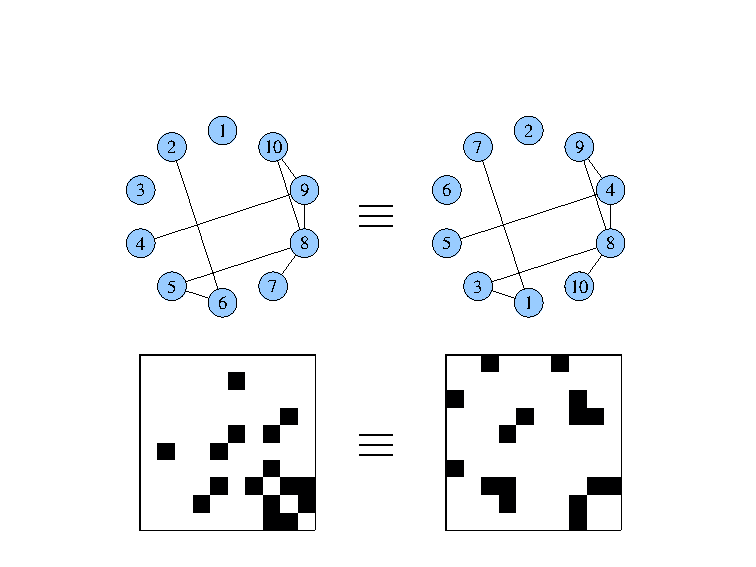
\includegraphics{figures/exchange}
\par\end{centering}

\caption{\label{fig:exchange_graph}This represents a particular permutation
of the labels of the vertices of a random graph. If the distribution
of the random graph is invariant under all such permutations then
it is jointly exchangeable.}


\end{figure}

\end{defn}
To build some intuition we consider a series of examples:
\begin{example}
$X_{ij}=0$ for $i<j$ is trivially jointly exchangeable, since every
distinct pair of units is disconnected.
\end{example}

\begin{example}
$X_{ij}=(j-i)\mod2$ is not jointly exchangeable.
\end{example}

\begin{example}
$X_{ij}\overset{iid}{\sim}\mbox{Bern}\left(p\right)$ is jointly exchangeable.
\end{example}

\begin{example}
$X_{ij}|p\overset{iid}{\sim}\mbox{Bern}\left(p\right)$ is jointly
exchangeable.
\end{example}

\begin{example}
\label{theta-random-ex}$X_{ij}|\boldsymbol{N}\overset{iid}{\sim}\mbox{Bern}\left(\sigma\left(\langle N_{i},N_{j}\rangle\right)\right)$,
where $N_{i}\overset{iid}{\sim}N\left(\mu,\Lambda\right)$, $\langle,\rangle$
denotes inner product and $\sigma:\mathbb{R}\rightarrow\left[0,1\right]$.
This model is also exchangeable. (nb. this is closely related to the
eigenmodel).
\end{example}
To state the representation theorem corresponding to this flavour
of exchangeability we will need one final definition:
\begin{defn}
Let $U_{1},U_{2},\dots$ be iid uniform random variables in $\left[0,1\right]$.
Let $\Theta:\left[0,1\right]^{2}\rightarrow\left[0,1\right]$ be a
symmetric measurable function and let 
\[
X_{ij}=1\mbox{ with probability }\Theta\left(U_{i},U_{j}\right)
\]
independently for all $i<j\in\mathbb{N}$. A \emph{$\Theta$-random
graph} is an array with the same distribution as $X$. A \emph{graphon}
is a symmetric measurable function from $\left[0,1\right]^{2}$ to
$\left[0,1\right]$. See figure \ref{fig:random_graph}.

\begin{figure}
\begin{centering}
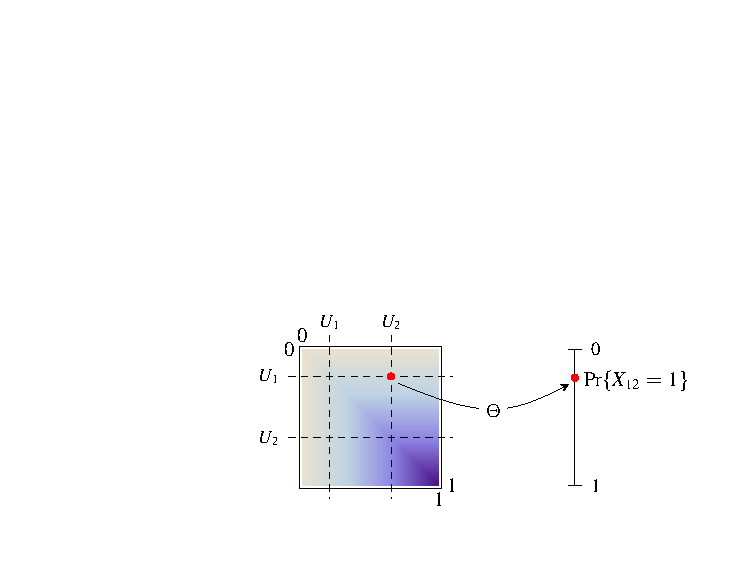
\includegraphics{figures/graphon1}
\par\end{centering}

\caption{\label{fig:random_graph}A pictorial representation of the construction
of a $\Theta$-random graph. $\Theta$ is defined on $\left[0,1\right]^{2}$
with value indicated by greyscale value. To determine the value of
$X_{ij}$ we select coordinates $U_{1}$ and $U_{2}$ then flip a
weighted coin with weight $\Theta\left(U_{1},U_{2}\right)$.}
\end{figure}

\end{defn}
Example \ref{theta-random-ex} is an example of a $\Theta$-random
graph, with 
\[
\Theta\left(\cdot,\cdot\right)=\sigma\left(\langle\Phi^{-1}\left(\cdot\right),\Phi^{-1}\left(\cdot\right)\rangle\right),
\]
where $\Phi^{-1}\left(\cdot\right)$ is the pseudo-inverse of the
$N\left(\mu,\Lambda\right)$ cumulative distribution function. That
is, $\Phi^{-1}\left(\cdot\right)$ is the function such that $\Phi^{-1}\left(U_{i}\right)\eqdist N_{i}$
where $U_{i}\sim U\left[0,1\right]$ and $N_{i}\sim N\left(\mu,\Lambda\right)$.
This example makes it clear that the choice of uniformly random variables
in the definition of $\Theta$-random graph is arbitrary: any atom-free
distribution%
\footnote{$g$ is atom free if $X_{1}\sim g$, $X_{2}\sim g\implies\Pr\left(X_{1}=X_{2}\right)=0$ %
} would work equally well.

It is easy to see that any $\Theta$-random graph\emph{ }is exchangeable.
The content of the representation theorem is that exchangeability
also implies that the graph is conditionally $\Theta$-random:
\begin{thm}
(Aldous, Hoover) Let $X=\left(X_{ij}\right)_{i,j\in\mathbb{N}}$ be
the adjacency matrix of an undirected graph on $\mathbb{N}$. The
following are equivalent:
\begin{enumerate}
\item $X$ is jointly exchangeable.
\item $X$ is conditionally $\Theta$-random, given a random graphon $\Theta$.
\end{enumerate}
\end{thm}
\begin{example}
Erdős-Renyi graphs are$\Theta$-random graphs with $\Theta\left(U_{i},U_{j}\right)=p$,
a constant function. 
\end{example}

\begin{example}
Let $Y_{1},Y_{2},\dots$ be a Pólya urn. Let $\phi:\mathbb{N}^{2}\rightarrow\mathbb{N}$
be a bijection and let $X_{ij}=Y_{\phi\left(i,j\right)}$. Then since
the Pólya urn is exchangeable we can conclude that the random graph
$X_{ij}$ is jointly exchangeable, and thus by the representation
theorem it is conditionally $\Theta$-random. In this case $\Theta\left(U_{i},U_{j}\right)=p,\ p\sim U\left[0,1\right]$.
\end{example}
We end by noting that in contrast to de Finetti's theorem the random
graphon of the Aldous-Hoover representation theorem is not unique.
To see this let $T:\left[0,1\right]\rightarrow\left[0,1\right]$ be
a transformation such that $T\left(U\right)\eqdist U$ and let
\[
\Theta^{T}\left(U_{1},U_{2}\right)=\Theta\left(T\left(U_{1}\right),T\left(U_{2}\right)\right).
\]
It is easy to see that $\Theta^{T}\eqdist\Theta$, thereby ruling
out uniqueness.
\end{document}
